\begin{figure} [H]
	\centering
	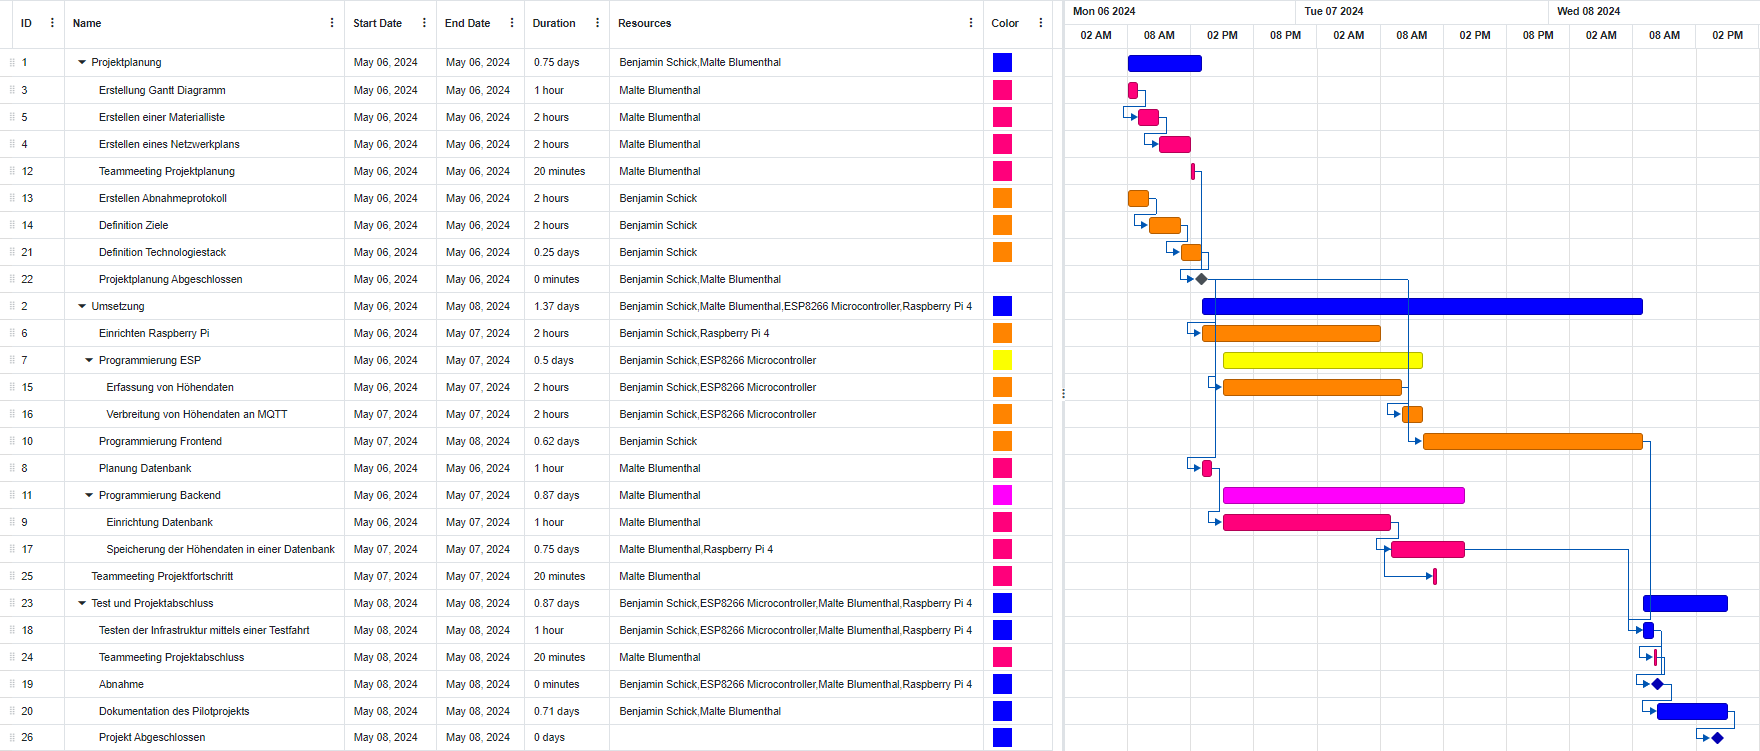
\includegraphics[width=15cm]{images/Zeitplanung.png}
	\caption[Terminplanung Tabellarisch]{Terminplanung Tabellarische Ansicht}
	\label{fig:terminplanung_tabellarisch}
\end{figure}

\begin{figure} [H]
	\centering
	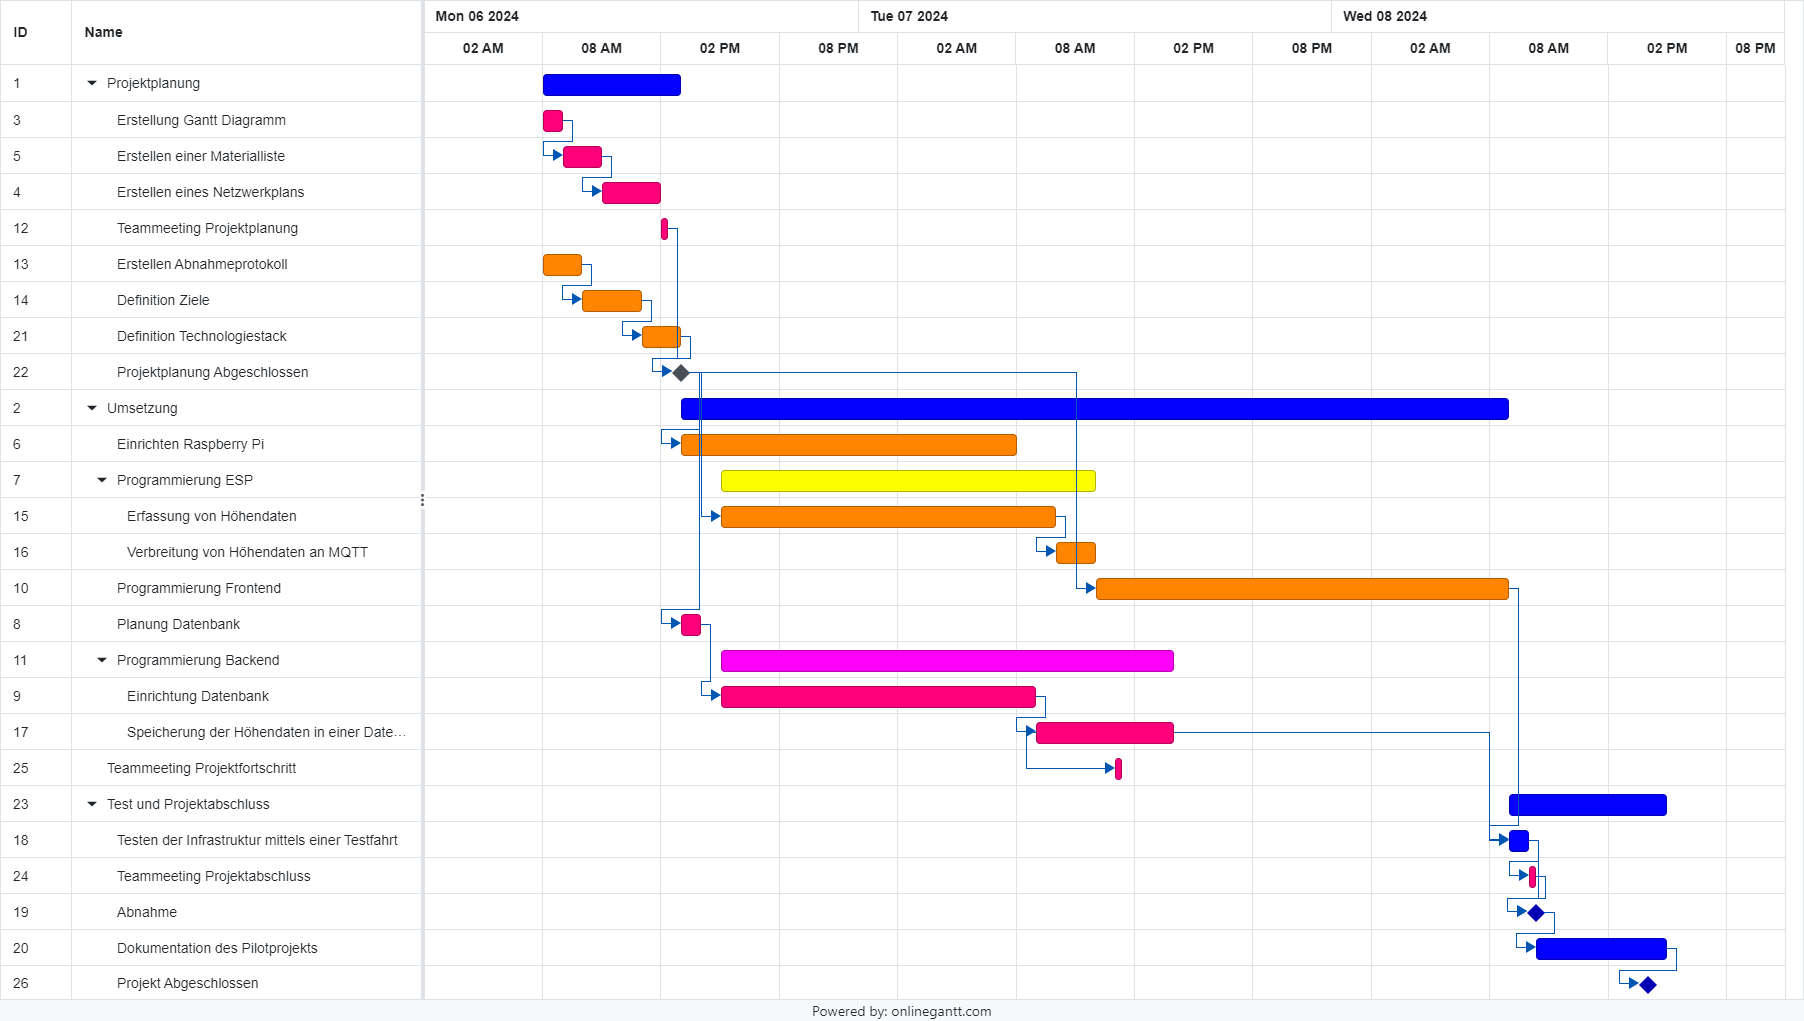
\includegraphics[width=15cm]{images/Gantt.png}
	\caption[Terminplanung Gantt]{Terminplanung Gantt-Diagramm}
	\label{fig:terminplanung_gantt}
\end{figure}

\begin{lstlisting}[language=C++,caption={WiFi connect}, label=lst:wificonnect]
	bool wifiConnect(String ssid, String password)
	{
		//Verbindung initialisieren
		WiFi.begin(ssid, password);
		
		//Debug-Ausgabe
		Serial.print("\nConnecting to: ");
		Serial.print(ssid);
		
		//Auf erfolgreiche Verbindung warten
		while (WiFi.status() != WL_CONNECTED) { // Wait for the Wi-Fi to connect
			Serial.print(".");
			delay(1000);
		}
		
		//Debug-Ausgabe
		Serial.print("\nConnection established. IP: ");
		Serial.println(WiFi.localIP());
		Serial.println("===================================");
		
		return true;
	}
\end{lstlisting}

\begin{lstlisting}[language=C++,caption={MQTT Connect}, label=lst:mqttconnect]
	bool brokerConnect(const char *address, int port)
	{
		//Serveradresse und -port setzen
		client.setServer(address, port);
		
		//ClientID erzeugen
		String clientId = "HurensohnClient-";
		clientId += String(random(0xffff), HEX);
		
		Serial.print("Attempting MQTT connection");
		
		//Konsequent versuchen, eine Verbindung herzustellen
		while (!client.connected()) 
		{
			//Verbindung hergestellt, Schleife verlassen
			if(client.connect(clientId.c_str()))
			{
				std::cout << "\nBroker "<< brokerAddress <<" connected\n" << std::endl;
				return true;
			}
			//Verbinden fehlgeschlagen, nach 1s erneut versuchen
			else
			{
				Serial.print(".");
				//Serial.println(client.state());
				delay(1000);
			}
		}
		return true;
	}
\end{lstlisting}

\begin{lstlisting}[language=C++,caption={Write Json}, label=lst:writejson]
	serializedData["device\_id"]   = ESP\_ID;
	serializedData["timestamp"]   = currData->timestamp;
	serializedData["temperature"] = currData->temperature;
	serializedData["humidity"]    = currData->humidity;
	serializedData["altitude"]    = currData->altitude;
	serializedData["airPressure"] = currData->airPressure;
\end{lstlisting}

\begin{figure}[H]
	\centering
	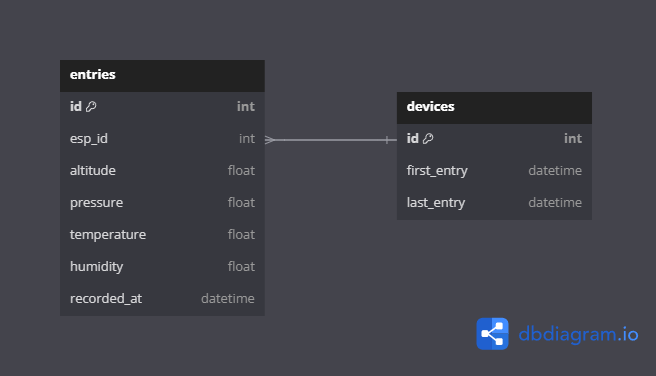
\includegraphics[width=15cm]{images/db_diagram.png}
	\caption{Datenbankdiagramm}
	\label{fig:db_diagram}
\end{figure}

\begin{lstlisting}[language=SQL, caption={Datenbankinitialisierungsscript}, label=lst:db_initialisation_script]
	DROP DATABASE esp_data;
	CREATE DATABASE IF NOT EXISTS esp_data;
	Use esp_data;
	
	DROP TABLE IF EXISTS devices;
	CREATE TABLE IF NOT EXISTS devices(
	id BIGINT UNSIGNED NOT NULL PRIMARY KEY UNIQUE,
	first_entry DATETIME,
	last_entry DATETIME
	);
	
	DROP TABLE IF EXISTS entries;
	CREATE TABLE IF NOT EXISTS entries(
	id BIGINT NOT NULL PRIMARY KEY AUTO_INCREMENT UNIQUE,
	esp_id BIGINT UNSIGNED NOT NULL,
	altitude FLOAT,
	pressure FLOAT,
	temperature FLOAT,
	humidity FLOAT,
	recorded_at DATETIME,
	FOREIGN KEY (esp_id) REFERENCES devices (id) ON DELETE RESTRICT ON UPDATE CASCADE
	);
\end{lstlisting}

\begin{lstlisting}[language=java, caption={Konfiguration der MariaDB Verbindung}, label=lst:conf_mariadb_conn]
	//MariaDB
	const mariadb = require('mariadb');
	const pool = mariadb.createPool({
		host: 'localhost',
		user: 'root',
		password: 'toor',
		database: 'esp_data',
		connectionLimit: 2
	});
\end{lstlisting}

\begin{lstlisting}[language=java, caption={Konfiguration der MQTT Verbindung}, label=lst:conf_mqtt_conn]
	//MQTT
	const mqtt = require('mqtt');
	const { each, error, ready } = require("jquery");
	const protocol = 'mqtt';
	const mqtt_broker = 'test.mosquitto.org';
	//const mqtt_broker = 'mqtt.eclipseprojects.io';
	const mqtt_port = 1883;
	const mqtt_url = protocol + '://' + mqtt_broker + ':' + mqtt_port;
	const mqtt_topic = 'est/katastrophenprojekt/espdaten';
	const mqtt_client = mqtt.connect(mqtt_url, keepalive = 60);
	let topic = mqtt_client.subscribe(mqtt_topic);
\end{lstlisting}

\begin{lstlisting}[language=java, caption={Event: MQTT Message}, label=lst:event_message]
	mqtt_client.on('message', (topic, message) => {
		console.log('Message:' + message);
		messageRecieved(message);
		//console.log('success');
	});
\end{lstlisting}

\begin{lstlisting}[language=java, caption={Funktion: messageRecieved}, label=lst:function_message_recieved]
	async function messageRecieved(message) {
		let conn;
		let jsonObj = JSON.parse(message);
		try {
			conn = await pool.getConnection();
			const res = await conn.query("INSERT INTO devices (id, first_entry, last_entry) VALUES (?, ?, ?) ON DUPLICATE KEY UPDATE last_entry = VALUES (last_entry);", [jsonObj.device_id, jsonObj.timestamp, jsonObj.timestamp]);
			console.log(res);
			const entry = await conn.query("INSERT INTO esp_data.entries (esp_id, altitude, pressure, temperature, humidity, recorded_at) VALUES (?, ?, ?, ?, ?, ?);", [jsonObj.device_id, jsonObj.altitude, jsonObj.airPressure, jsonObj.temperature, jsonObj.humidity, jsonObj.timestamp]);
			console.log(entry);
		} catch(err) {
			console.log("Error: " + err);
			throw err;
		}
		finally {
			if(conn) return conn.end();
		}
	}
\end{lstlisting}

\begin{lstlisting}[language=java, caption={Route: getData}, label=lst:route_get_data]
	app.get("/data", (req, res) => {
		readData(req, res);
	});
\end{lstlisting}

\begin{lstlisting}[language=java, caption={Funktion: readData}, label=lst:function_read_data]
	async function readData(req, res) {
		let conn;
		try {
			conn = await pool.getConnection();
			data = await conn.query("SELECT * FROM (SELECT * FROM entries ORDER BY recorded_at DESC LIMIT 1000) AS subquery ORDER BY id ASC;");
			res.json(data);
		} catch (err) {
			throw err;
		} finally {
			if (conn) conn.end();
		}
	}
\end{lstlisting}